\documentclass[12pt,a4paper]{report}

% --- Packages ---
\usepackage{times}           % Times New Roman
\usepackage{setspace}        % Line spacing
\usepackage{geometry}        % Margins
\usepackage{graphicx}        % Figures
\usepackage{booktabs}        % Professional tables
\usepackage{tabularx}        % Flexible tables
\usepackage{caption}         % Figure/table captions
\usepackage{subcaption}      % Subfigures
\usepackage{listings}        % Code listings
\usepackage{amsmath}         % Math equations
\usepackage{hyperref}        % Hyperlinks in PDF
\usepackage{fancyhdr}        % Headers/footers
\usepackage{titlesec}        % Section title formatting
\usepackage{ragged2e}        % Justification

% --- Geometry ---
\geometry{top=1in, bottom=1in, left=1.5in, right=1in}

% --- Spacing ---
\onehalfspacing

% --- Title formatting ---
% Chapter title: 18pt Bold Centered
\titleformat{\chapter}[display]
  {\normalfont\fontsize{18}{22}\bfseries\centering}
  {Chapter \thechapter}{20pt}{}

% Section (Heading 2): 16pt Bold Left
\titleformat{\section}
  {\normalfont\fontsize{16}{20}\bfseries}
  {\thesection}{1em}{}

% Subsection (Heading 3): 14pt Bold Left
\titleformat{\subsection}
  {\normalfont\fontsize{14}{18}\bfseries}
  {\thesubsection}{1em}{}

% --- Code listings styling ---
\lstdefinelanguage{RISCV}{
  morekeywords={addi,sw,lw,jal,jalr,jr,la,li,bne,blt,add,sub,nop,j},
  sensitive=false,
  morecomment=[l]{\#},
}
\lstset{
  language=RISCV,
  basicstyle=\ttfamily\small,
  keywordstyle=\bfseries,
  commentstyle=\itshape,
  numbers=left,
  numberstyle=\tiny,
  frame=single,
  breaklines=true,
  captionpos=b
}

% --- Header/Footer ---
\pagestyle{fancy}
\fancyhf{}
\rhead{\textit{Buffer Overflow and Control Hazards in RISC-V}}
\lhead{\textit{NSS College of Engineering, Palakkad}}
\cfoot{\thepage}

% --- Document begins ---
\begin{document}

\input{titlepage}
\begin{center}
{\Large \bfseries NSS COLLEGE OF ENGINEERING, PALAKKAD}\\[0.5cm]
{\large \bfseries Department of Computer Science and Engineering}\\[1.5cm]
{\LARGE \bfseries CERTIFICATE}\\[1.5cm]
\end{center}
\begin{flushleft}
This is to certify that the project report entitled 
\textbf{"Buffer Overflow and Control Hazards in RISC-V Architecture"} 
is a bonafide record of the work done by Group No. 4:\\[0.5cm]

\textbf{Adharsh K \quad (Register No: NSS24CS010)}\\
\textbf{Angelino Saul \quad (Register No: NSS24CS036)}\\
\textbf{Aswin Manoj \quad (Register No: NSS24CS054)}\\
\textbf{Aswin R \quad (Register No: NSS24CS055)}\\[0.5cm]

under our guidance during the academic year 2025--2026.
\end{flushleft}

\vspace{3cm}

\noindent
\begin{tabular}{@{}p{0.5\textwidth}p{0.5\textwidth}@{}}
\textbf{Signature of Guide} & \textbf{Signature of HOD} \\
Name: Reshma S & Name: Anuraj Mohan \\
Date: & Date: \\
\end{tabular}
\thispagestyle{empty}
\newpage

\chapter*{Acknowledgement}
\addcontentsline{toc}{chapter}{Acknowledgement}

We express our sincere gratitude to \textbf{Reshma S}, our project guide, for their valuable guidance and support throughout this project. 

We thank the Department of Computer Science and Engineering, NSS College of Engineering, Palakkad, for providing access to the necessary tools and resources. 

We also acknowledge the open-source Ripes simulator project for enabling practical RISC-V pipeline analysis.
\newpage

\chapter*{Abstract}
\addcontentsline{toc}{chapter}{Abstract}

This project analyzes the impact of buffer overflow vulnerabilities on the RISC-V processor pipeline. Utilizing the Ripes simulator, the study models a 5-stage RISC-V pipeline executing a custom RISC-V assembly program designed with a vulnerable function. The objective is to bridge the gap between theoretical memory mapping and practical instruction-level execution.

By intentionally overwriting the saved return address (\texttt{ra}) on the stack, the experiment demonstrates how a memory corruption vulnerability can escalate into a control flow subversion. The findings show that an overflow at \texttt{sp+12} corrupts the return address from its legitimate value (\texttt{0x00000004}) to a target address (\texttt{0x00000034}), successfully hijacking the program counter (PC) to execute a hidden code segment. Furthermore, the analysis reveals that this attack incurs a 2-cycle control hazard penalty as the processor pipeline resolves the \texttt{jr ra} instruction during the Execution (EX) stage.

\vspace{1cm}
\noindent\textbf{Keywords:} Buffer Overflow, RISC-V, Stack-Based Attack, Return Address, Control Hazard, Pipeline Flush, Ripes Simulator
\newpage


\tableofcontents

\clearpage
\phantomsection
\addcontentsline{toc}{chapter}{\listfigurename}
\listoffigures

\clearpage
\phantomsection
\addcontentsline{toc}{chapter}{\listtablename}
\listoftables

\chapter{Introduction}

\section{Background and Motivation}
Modern processors rely heavily on pipelining to increase instruction throughput and improve overall system performance. However, security vulnerabilities at the instruction level can uniquely affect architectural behavior. A classic example is the buffer overflow, which remains a historical and ongoing real-world threat to system integrity. By deeply analyzing how a buffer overflow manipulates processor state, we can understand the connection between high-level vulnerabilities and hardware-level execution. The Ripes simulator provides an invaluable platform for this, allowing architectural-level observation that is not possible in high-level languages like C or Python.

\section{Problem Statement}
\textit{"The core problem is to bridge the gap between theoretical concepts of memory mapping, instruction execution, and pipeline hazards with a practical demonstration of how vulnerabilities at the instruction level can propagate through processor stages and affect overall system behavior."}

\section{Objectives}
The key objectives of this study are:
\begin{itemize}
    \item To practically demonstrate a buffer overflow vulnerability at the instruction level using RISC-V assembly.
    \item To observe how a corrupted return address hijacks the processor's control flow.
    \item To trace the resulting control hazard through a 5-stage instruction pipeline.
    \item To quantify the pipeline penalty incurred by the illicit branch execution.
\end{itemize}

\section{Study Scope and Constraints}
This study is conducted under specific constraints to isolate the architectural effects:
\begin{itemize}
    \item \textbf{Simulator:} Ripes v2.x, configured with a 5-stage pipelined processor.
    \item \textbf{ISA:} RV32IM (32-bit RISC-V integer and multiplication instruction set).
    \item \textbf{Attack Type:} Stack-based return address overwrite.
    \item \textbf{Environment Context:} The simulation runs bare-metal with no Operating System (OS) or memory cache modelling.
    \item \textbf{Nature of Exploit:} The overflow is controlled and intentionally induced via assembly logic, not through external user input or accidental bounds violation.
\end{itemize}

\section{Report Structure}
The rest of this report is organized as follows: Chapter 2 discusses the theoretical background, including the RISC-V stack architecture, pipelining, and buffer overflow mechanics. Chapter 3 details the methodology and experimental setup. Chapter 4 presents the results observed in the Ripes simulator. Chapter 5 discusses the implications and potential mitigations, followed by the conclusion in Chapter 6.

\chapter{Theoretical Background}

\section{Memory and Stack Architecture in RISC-V}
In the RISC-V architecture, the stack traditionally grows downwards, meaning the stack pointer (\texttt{sp}) decreases as memory is allocated. A typical stack frame layout consists of local buffers, padding, and the saved return address (\texttt{ra}). For a frame containing a 2-word buffer and the saved return address:
\begin{itemize}
    \item \texttt{sp+0} = \texttt{buf[0]}
    \item \texttt{sp+4} = \texttt{buf[1]}
    \item \texttt{sp+12} = \texttt{saved\_ra}
\end{itemize}

\begin{table}[h]
\caption{Example Stack Frame Mapping}
\centering
\begin{tabular}{|l|l|l|}
\hline
\textbf{Offset} & \textbf{Address (example)} & \textbf{Contents} \\
\hline
\texttt{sp+0} & \texttt{0x7fffffe0} & \texttt{buf[0] = 10} \\
\texttt{sp+4} & \texttt{0x7fffffe4} & \texttt{buf[1] = 10} \\
\texttt{sp+8} & \texttt{0x7fffffe8} & (unused/padding) \\
\texttt{sp+12} & \texttt{0x7fffffec} & saved \texttt{ra} (TARGET) \\
\hline
\end{tabular}
\label{tab:stack_map}
\end{table}

\section{The 5-Stage Pipeline}
Pipelining allows multiple instructions to be processed simultaneously. The standard 5-stage RISC-V pipeline consists of the following stages:

\begin{table}[h]
\caption{The 5 Stages of the Processor Pipeline}
\centering
\begin{tabular}{|l|l|p{8cm}|}
\hline
\textbf{Stage} & \textbf{Name} & \textbf{Description} \\
\hline
IF & Instruction Fetch & Fetches the instruction from memory using the PC. \\
ID & Instruction Decode & Decodes the instruction and reads registers. \\
EX & Execution & ALU performs arithmetic or resolves branch conditions/targets. \\
MEM & Memory Access & Reads or writes data to/from data memory. \\
WB & Write Back & Writes the result back to the register file. \\
\hline
\end{tabular}
\label{tab:pipeline}
\end{table}

\section{Pipeline Hazards}
Hazards prevent the next instruction in the instruction stream from executing during its designated clock cycle. There are three primary types of pipeline hazards:

\begin{table}[h]
\caption{Types of Pipeline Hazards}
\centering
\begin{tabular}{|l|p{10cm}|}
\hline
\textbf{Hazard Type} & \textbf{Description} \\
\hline
Structural Hazard & Hardware cannot support the combination of instructions needed in the same clock cycle. \\
Data Hazard & Instruction depends on the results of a previous instruction still in the pipeline. \\
Control Hazard & Caused by a delay in determining the proper target address of a branch or jump. \\
\hline
\end{tabular}
\label{tab:hazards}
\end{table}

\section{Control Hazards and Branch Flush Penalty}
Control hazards occur when the pipeline makes the wrong decision on branch prediction and fetches instructions that shouldn't be executed. In the tested RISC-V pipeline, branches resolve at the Execution (EX) stage. If a branch is taken, the instructions already loaded into the IF and ID stages must be flushed, resulting in a \textbf{2-cycle penalty} (Formula: Penalty = 2 cycles per taken branch).

\begin{table}[h]
\caption{Pipeline Trace for a Control Hazard on \texttt{jr ra}}
\centering
\begin{tabular}{|l|c|c|c|c|c|}
\hline
\textbf{Instruction} & \textbf{C1} & \textbf{C2} & \textbf{C3} & \textbf{C4} & \textbf{C5} \\
\hline
\texttt{jr ra} & IF & ID & EX & MEM & WB \\
Fetch+1 & & IF & flush & & \\
Fetch+2 & & & IF & flush & \\
\texttt{secret[0]} & & & & IF & ID \\
\hline
\end{tabular}
\label{tab:hazard_trace}
\end{table}

\section{Buffer Overflow: Definition and Classification}
According to NIST, a buffer overflow occurs when a program attempts to put more data in a memory buffer than it can hold, leading to memory corruption. Vulnerabilities are generally classified into heap-based and stack-based overflows. In our study, we focus on a stack-based buffer overflow, specifically targeting \texttt{sp+12}, where the architecture stores the return address (\texttt{ra}) for function calls.

\section{Stack-Based Buffer Overflow Mechanics}
During normal execution, data is written exclusively to the allocated space (e.g., \texttt{sp+0} and \texttt{sp+4}). A stack-based overflow occurs when a write operation bypasses these bounds, writing to adjacent memory addresses. When an attacker intentionally writes to \texttt{sp+12}, they overwrite the saved \texttt{ra}, effectively changing the control return path.

\section{Return Address Corruption and PC Hijack}
In RISC-V, the return address registers (\texttt{x1} or \texttt{ra}) hold the address to return to after a subroutine completes. A subroutine call (\texttt{jal}) writes \texttt{PC+4} to \texttt{ra}. If the stack memory corresponding to the saved \texttt{ra} is overwritten, the \texttt{lw ra, 12(sp)} instruction during the function epilogue will load a corrupted value. Consequently, when the \texttt{jr ra} instruction executes, the Program Counter (PC) jumps to the illicit address, effectively hijacking control flow of the processor.

\chapter{Methodology}

\section{Experimental Setup (Ripes Configuration)}
The experiment utilizes the Ripes simulator to visualize instruction execution and pipeline flow. Ripes is configured as follows:
\begin{itemize}
    \item \textbf{Processor:} 5-Stage Pipelined
    \item \textbf{ISA:} RV32IM
    \item \textbf{Data Forwarding:} Default enabled
    \item \textbf{Branch Prediction:} None
\end{itemize}

\begin{figure}[h]
  \centering
  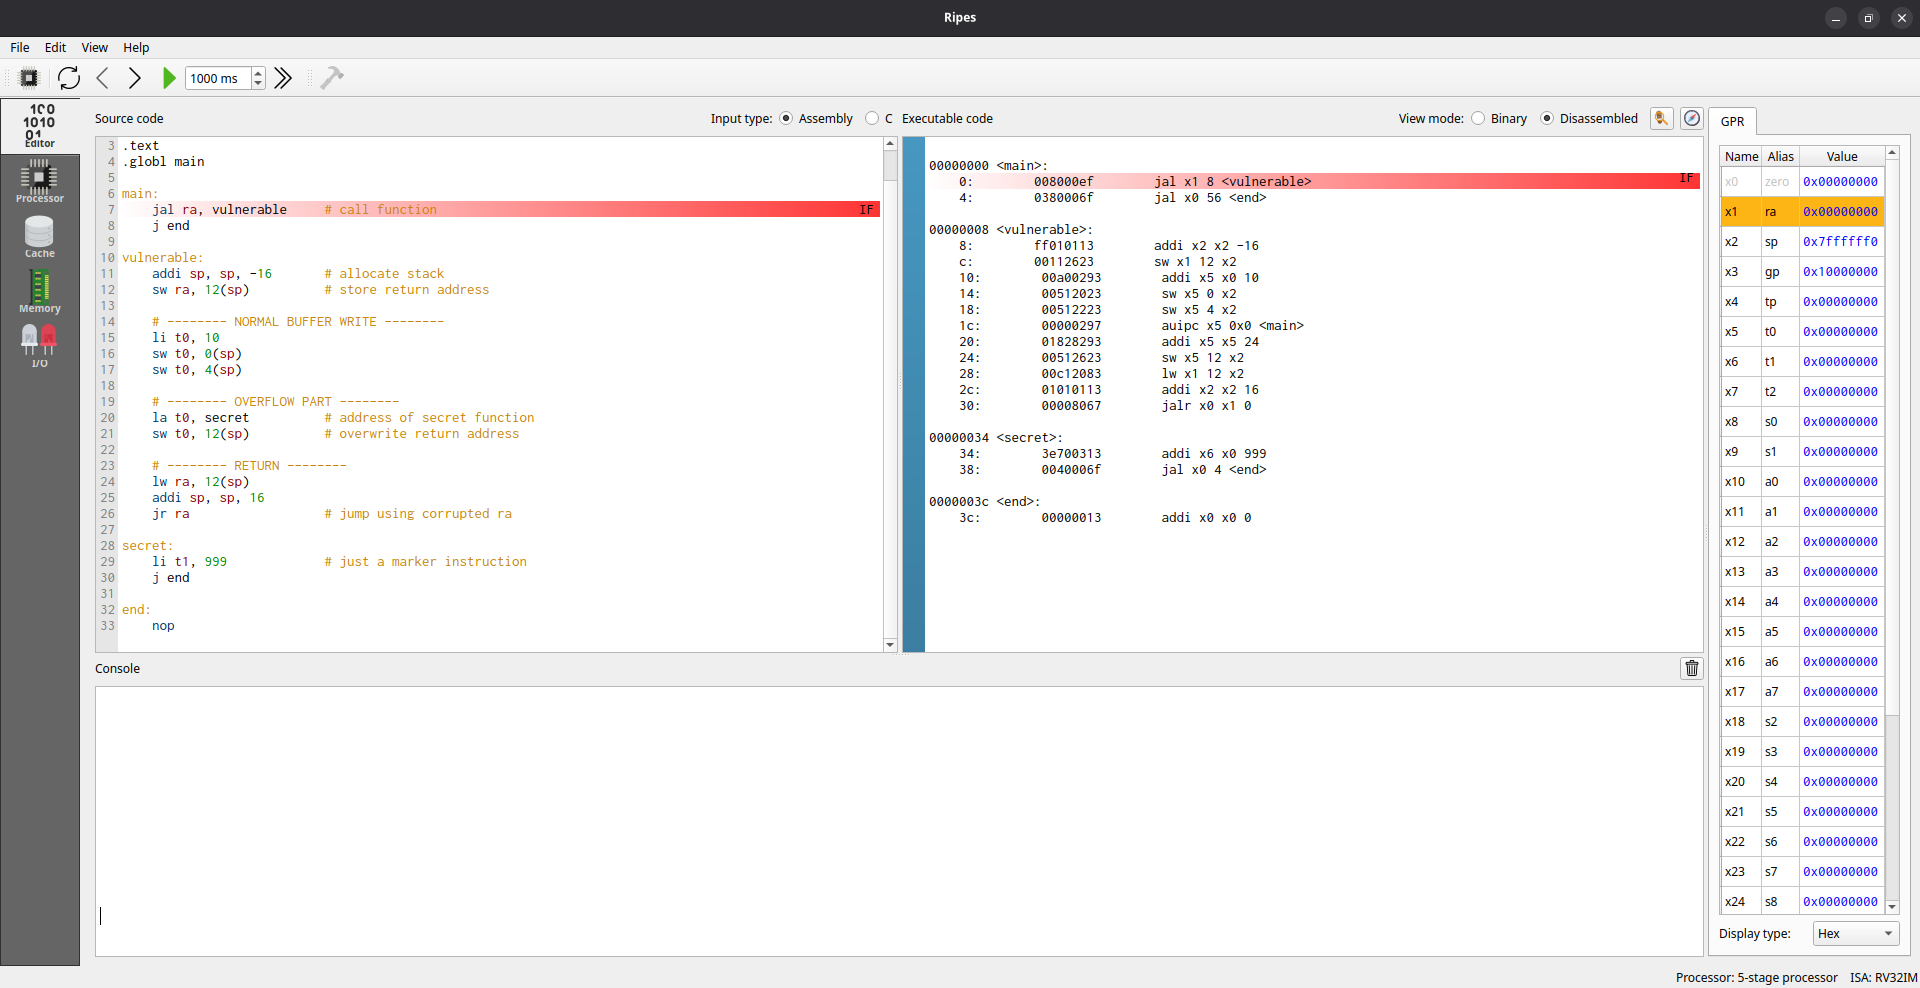
\includegraphics[width=0.8\textwidth]{images/ss1.png}
  \caption{Ripes simulator with 5-stage processor and program loaded.}
  \label{fig:ss1}
\end{figure}

\section{Program Design and Logic}
A specific RISC-V assembly program was crafted to model the attack. It contains a \texttt{main} routine, a \texttt{vulnerable} function which allocates a stack frame, and a hidden \texttt{secret} function. The complete annotated code represents the target application:

\begin{lstlisting}[language=RISCV, caption={Vulnerable RISC-V Assembly Program}]
.text
.globl main

main:
    jal ra, vulnerable      # call function; ra = addr of "j end"
    j end

vulnerable:
    addi sp, sp, -16        # allocate 16-byte stack frame
    sw ra, 12(sp)           # save legitimate return address

    # Normal buffer writes
    li t0, 10
    sw t0, 0(sp)            # buf[0] = 10
    sw t0, 4(sp)            # buf[1] = 10

    # Overflow: overwrite saved return address
    la t0, secret
    sw t0, 12(sp)           # OVERFLOW: saved ra -> address of secret

    # Return using corrupted ra
    lw ra, 12(sp)           # ra = address of secret (corrupted)
    addi sp, sp, 16
    jr ra                   # PC hijacked -> jumps to secret

secret:
    li t1, 999              # marker: proves execution reached here
    j end

end:
    nop
\end{lstlisting}

\section{Stack Memory Map}
The program allocates 16 bytes for the stack frame. The logical mapping is presented below, illustrating how the 12-byte offset creates a clear path to the return address:

\begin{table}[h]
\caption{Memory Layout within the \texttt{vulnerable} Function}
\centering
\begin{tabular}{|l|l|l|}
\hline
\textbf{Offset} & \textbf{Address (Absolute)} & \textbf{Data Purpose} \\
\hline
\texttt{sp+0} & \texttt{0x7fffffe0} & Buffer data \\
\texttt{sp+4} & \texttt{0x7fffffe4} & Buffer data \\
\texttt{sp+8} & \texttt{0x7fffffe8} & Unused \\
\texttt{sp+12} & \texttt{0x7fffffec} & Saved Return Address \\
\hline
\end{tabular}
\label{tab:methodology_stack}
\end{table}

\section{Instruction Flow Design}
The logical progression of the exploit follows six core phases based on instruction execution:
\begin{enumerate}
    \item Function setup via \texttt{jal}.
    \item Stack frame allocation and valid return address anchoring via \texttt{sw ra, 12(sp)}.
    \item Standard buffer manipulation via localized stores.
    \item The exploit trigger: a \texttt{sw} instruction explicitly targeting \texttt{12(sp)} with the address of \texttt{secret}.
    \item Corrupted context restoration via \texttt{lw ra, 12(sp)}.
    \item Control subversion via \texttt{jr ra}, violating intended control flow.
\end{enumerate}

\section{Measurement Procedure}
The procedural steps for running the test are:
\begin{enumerate}
    \item Load the compiled program into the Ripes simulator.
    \item Single-step the execution to monitor precise architectural state changes.
    \item Monitor the register panel for the value of \texttt{x1} (\texttt{ra}).
    \item Monitor the memory panel for the hex values at the dynamic stack address coordinates.
    \item Examine the pipeline diagram specifically during the execution of jump/branch instructions to identify flush conditions.
    \item Capture the architectural state at each critical instruction to record empirical evidence of the attack chain.
\end{enumerate}

\chapter{Results and Observations}

\section{Normal Stack Setup}
Following the \texttt{jal} instruction into the \texttt{vulnerable} function, a 16-byte stack frame is allocated. The \texttt{sw ra, 12(sp)} instruction executes normally. In the register panel, \texttt{ra} (\texttt{x1}) holds the legitimate return value \texttt{0x00000004}. Correspondingly, the memory at \texttt{sp+12} is anchored precisely at \texttt{0x00000004}. At this point, the pipeline displays all five stages operating under normal IF/ID/EX/MEM/WB sequences.

\begin{figure}[h]
  \centering
  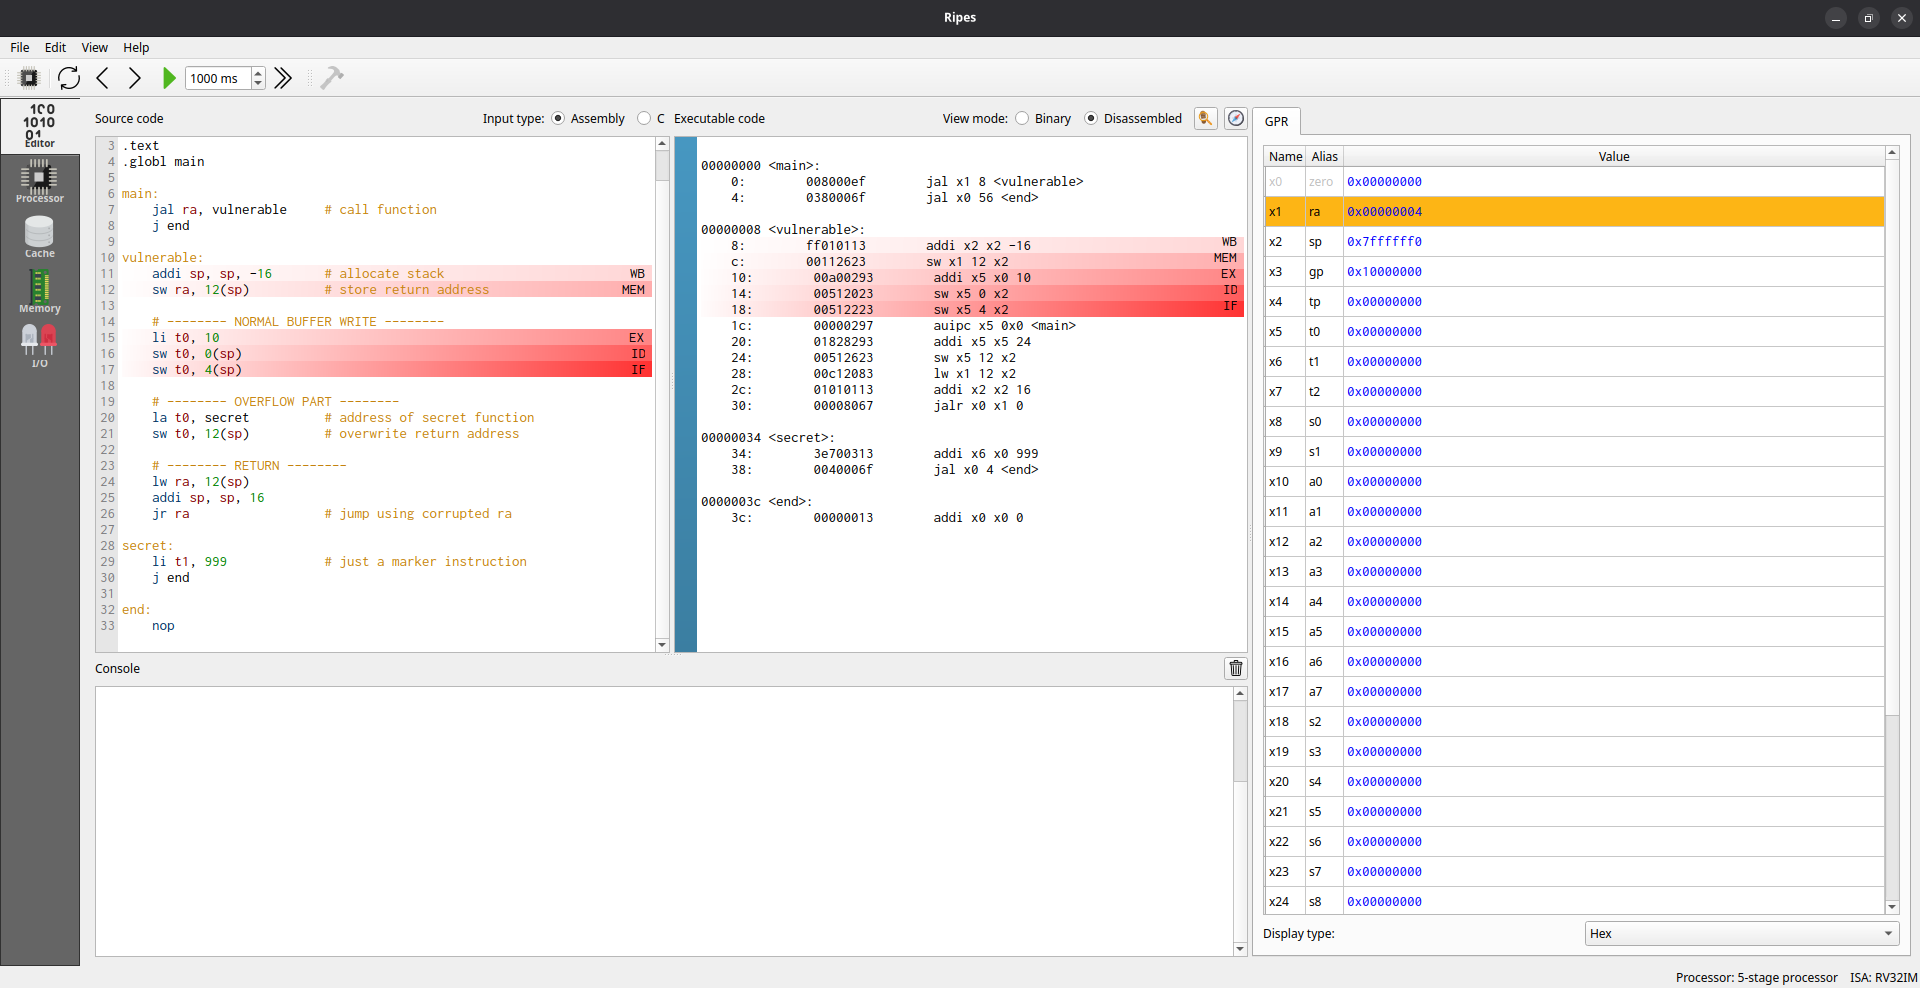
\includegraphics[width=0.8\textwidth]{images/ss2.png}
  \caption{Register file showing \texttt{ra=0x00000004} after legitimate save.}
  \label{fig:ss2}
\end{figure}

\section{Buffer Write Phase}
The standard buffer writes execute next: \texttt{sw t0, 0(sp)} and \texttt{sw t0, 4(sp)}. Memory observations confirm that \texttt{sp+0} and \texttt{sp+4} now contain \texttt{0x0000000A} (the value 10). Crucially, the target slot at \texttt{sp+12} remains intact with the value \texttt{0x00000004}.

\section{The Overflow Event}
The critical simulated breach occurs at the execution of \texttt{sw t0, 12(sp)}. The instruction proceeds to the MEM stage where it overwrites the architectural return slot. 

\begin{figure}[h]
  \centering
  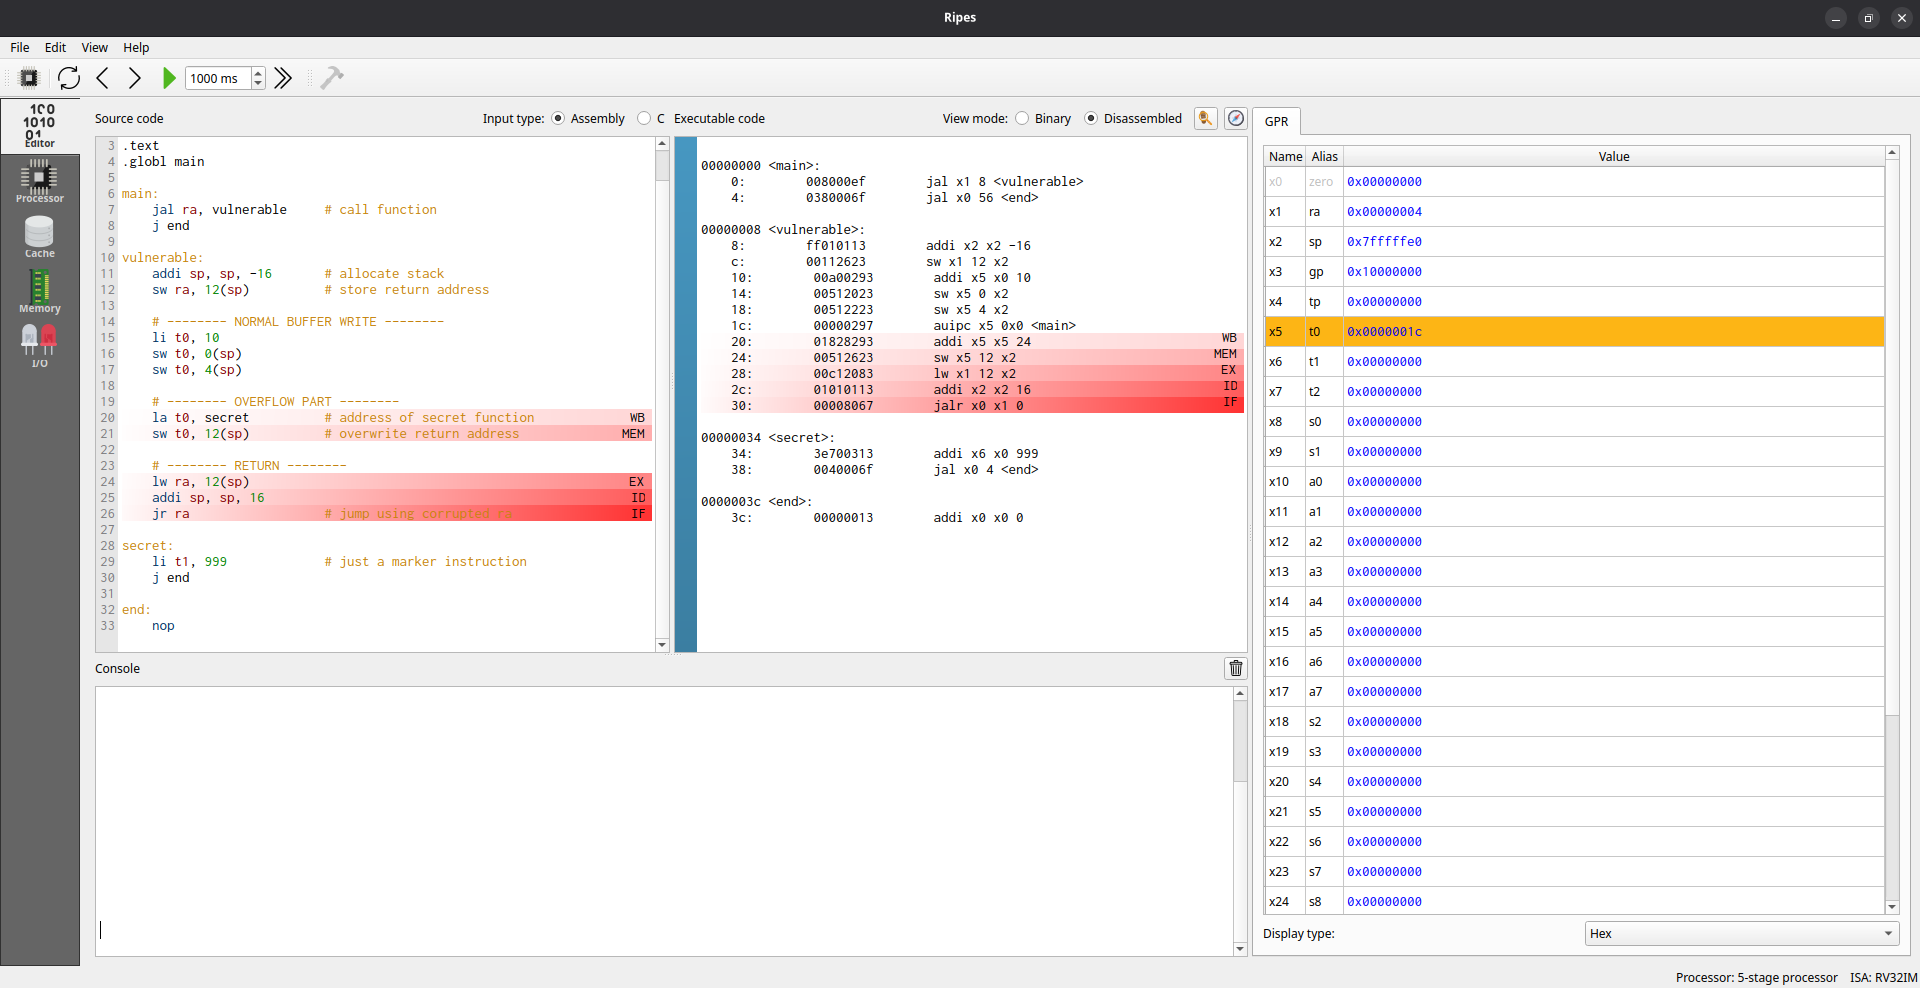
\includegraphics[width=0.8\textwidth]{images/ss3.png}
  \caption{\texttt{sw t0,12(sp)} in MEM stage --- overflow instruction executing.}
  \label{fig:ss3}
\end{figure}

Memory observation immediately highlights that \texttt{sp+12} has changed from \texttt{0x00000004} to \texttt{0x00000034} (the address of our \texttt{secret} function). This constitutes the core buffer overflow: a protected memory location is destructively overwritten.

\section{Return Address Corruption}
During the function epilogue, the \texttt{lw ra, 12(sp)} instruction restores the context. However, because memory was corrupted, the register file reads the overwritten value. The state of \texttt{ra} (\texttt{x1}) shifts from \texttt{0x00000004} to \texttt{0x00000034}. 

\begin{figure}[h]
  \centering
  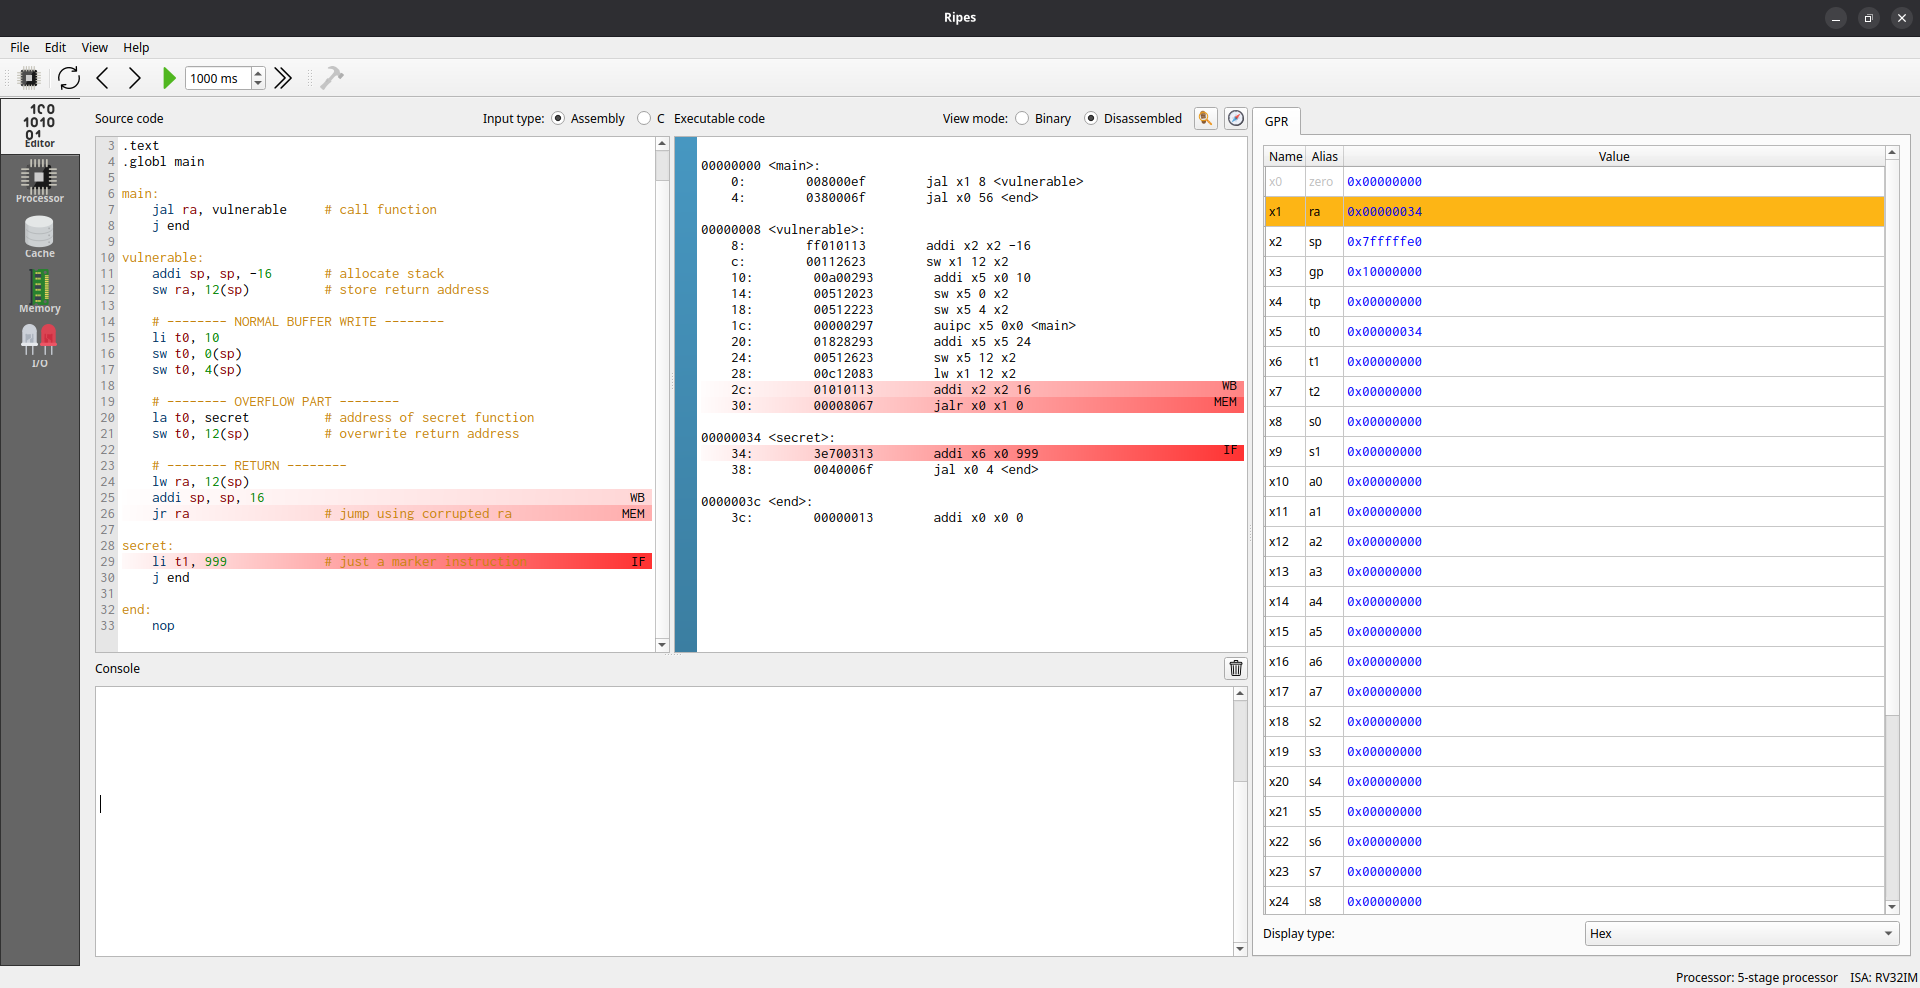
\includegraphics[width=0.8\textwidth]{images/ss4.png}
  \caption{\texttt{ra} corrupted to \texttt{0x00000034}; \texttt{li t1,999} is the current instruction.}
  \label{fig:ss4}
\end{figure}

\section{PC Hijack via \texttt{jr ra}}
The consequence of the corrupted return address manifests via the \texttt{jr ra} instruction. Instead of returning control to \texttt{main}, the Program Counter explicitly jumps to \texttt{0x00000034}. Execution of \texttt{li t1, 999} operates as empirical proof that code inside the \texttt{secret} function is currently executing. The normal intended path (\texttt{main} $\rightarrow$ \texttt{vulnerable} $\rightarrow$ \texttt{main}) is transformed into the hijacked path (\texttt{main} $\rightarrow$ \texttt{vulnerable} $\rightarrow$ \texttt{secret}).

\section{Control Hazard in the Pipeline}
Monitoring the Ripes pipeline diagram exposes a critical effect on dynamic scheduling. The \texttt{jr ra} instruction resolves in the EX stage. Due to the branch, speculative fetches—such as \texttt{li t1, 999} in ID, and \texttt{j end} in IF—are fed into the pipeline. This introduces a control hazard where the processor cannot determine the target natively until EX finishes. Consequently, a 2-cycle penalty is incurred as these instructions represent the inadvertently accepted path.

\begin{figure}[h]
  \centering
  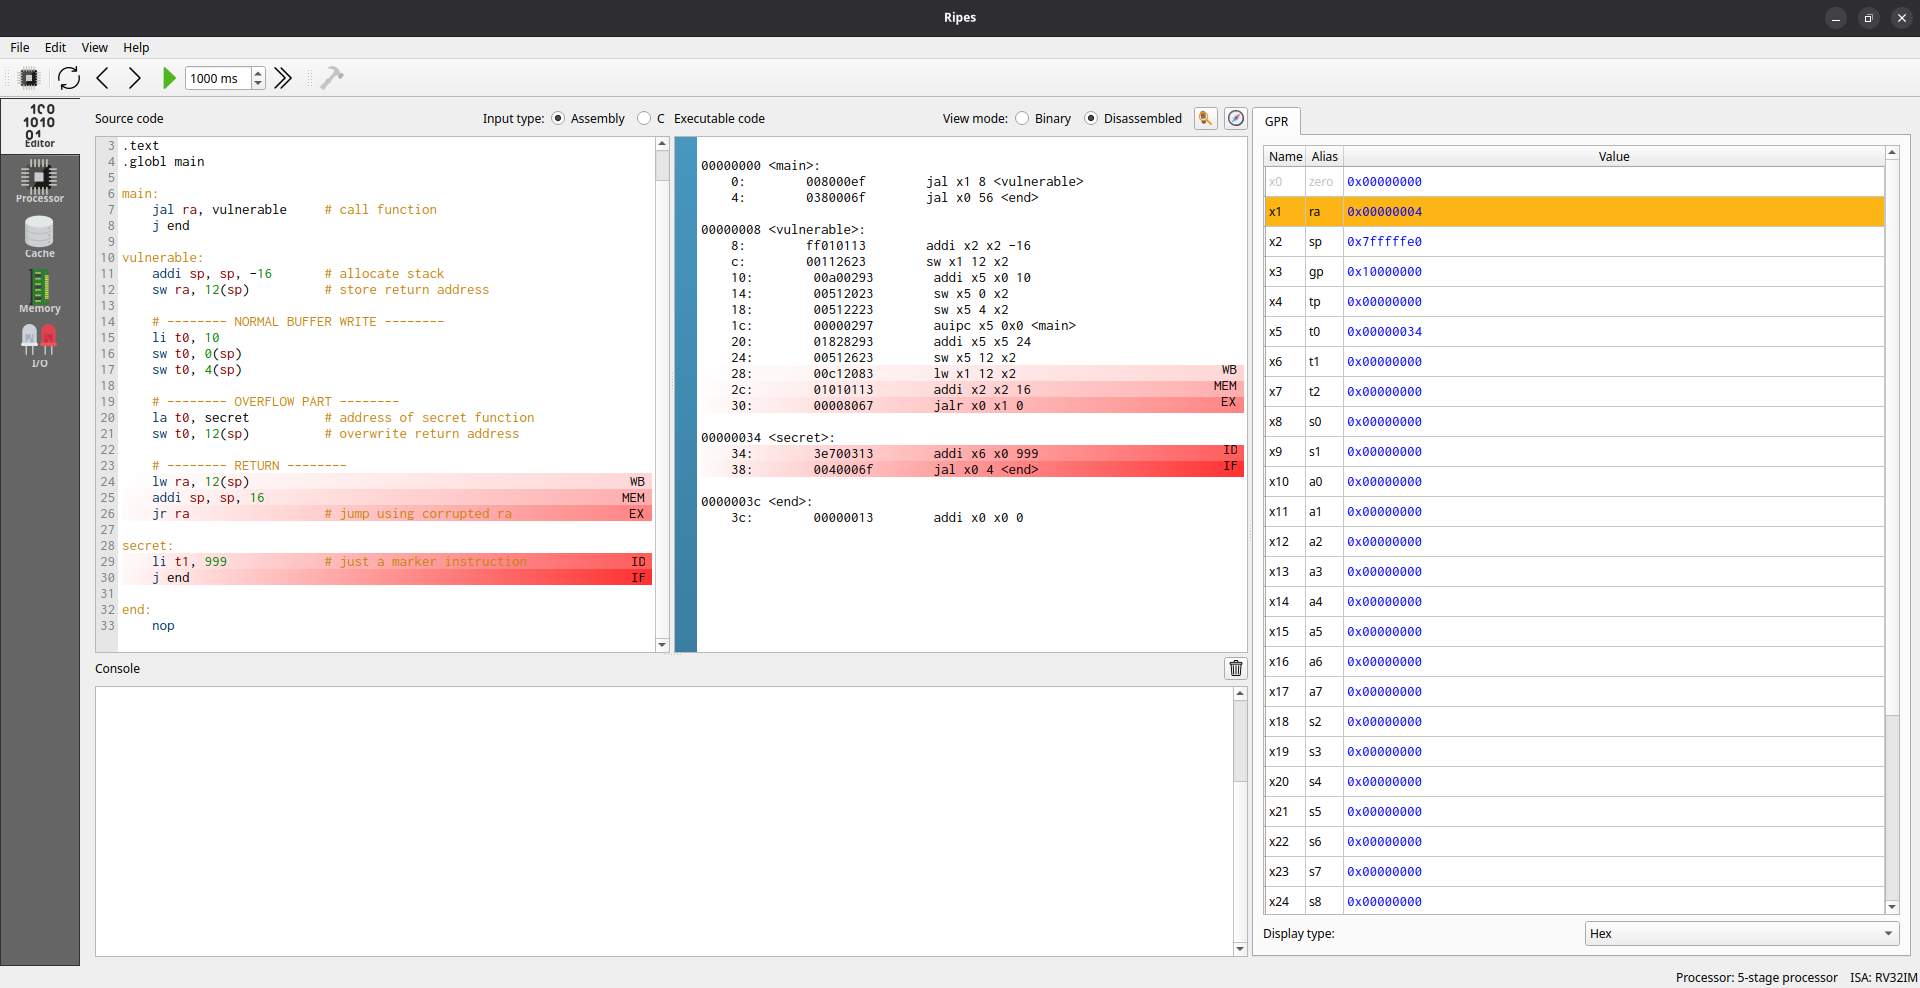
\includegraphics[width=0.8\textwidth]{images/ss5.png}
  \caption{\texttt{jr ra} in EX stage; \texttt{secret} instructions in ID and IF.}
  \label{fig:ss5}
\end{figure}

\section{Memory Comparison (Before vs After)}
The pre-condition and post-condition memory dumps reinforce the precision of the attack vector.

\begin{figure}[h]
  \centering
  \begin{minipage}{0.48\textwidth}
    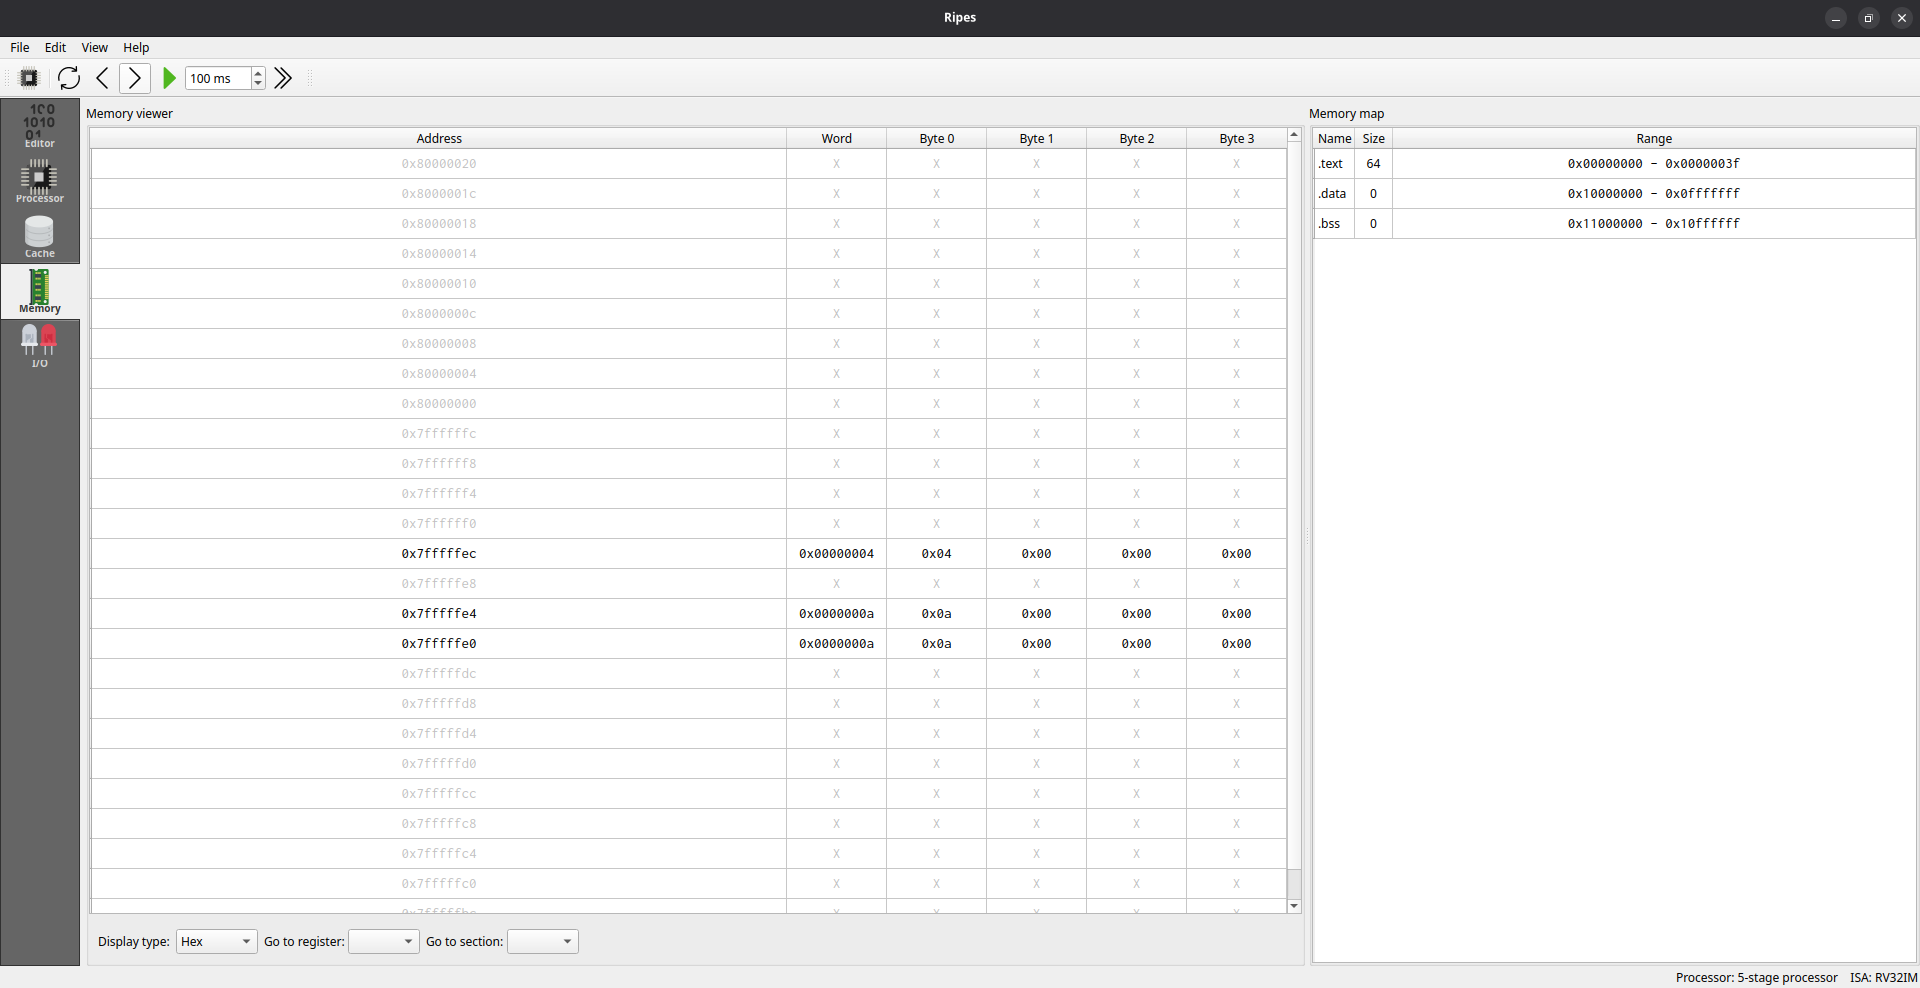
\includegraphics[width=\textwidth]{images/memory_before.png}
    \caption*{Before: \texttt{sp+12 = 0x00000004}}
  \end{minipage}
  \hfill
  \begin{minipage}{0.48\textwidth}
    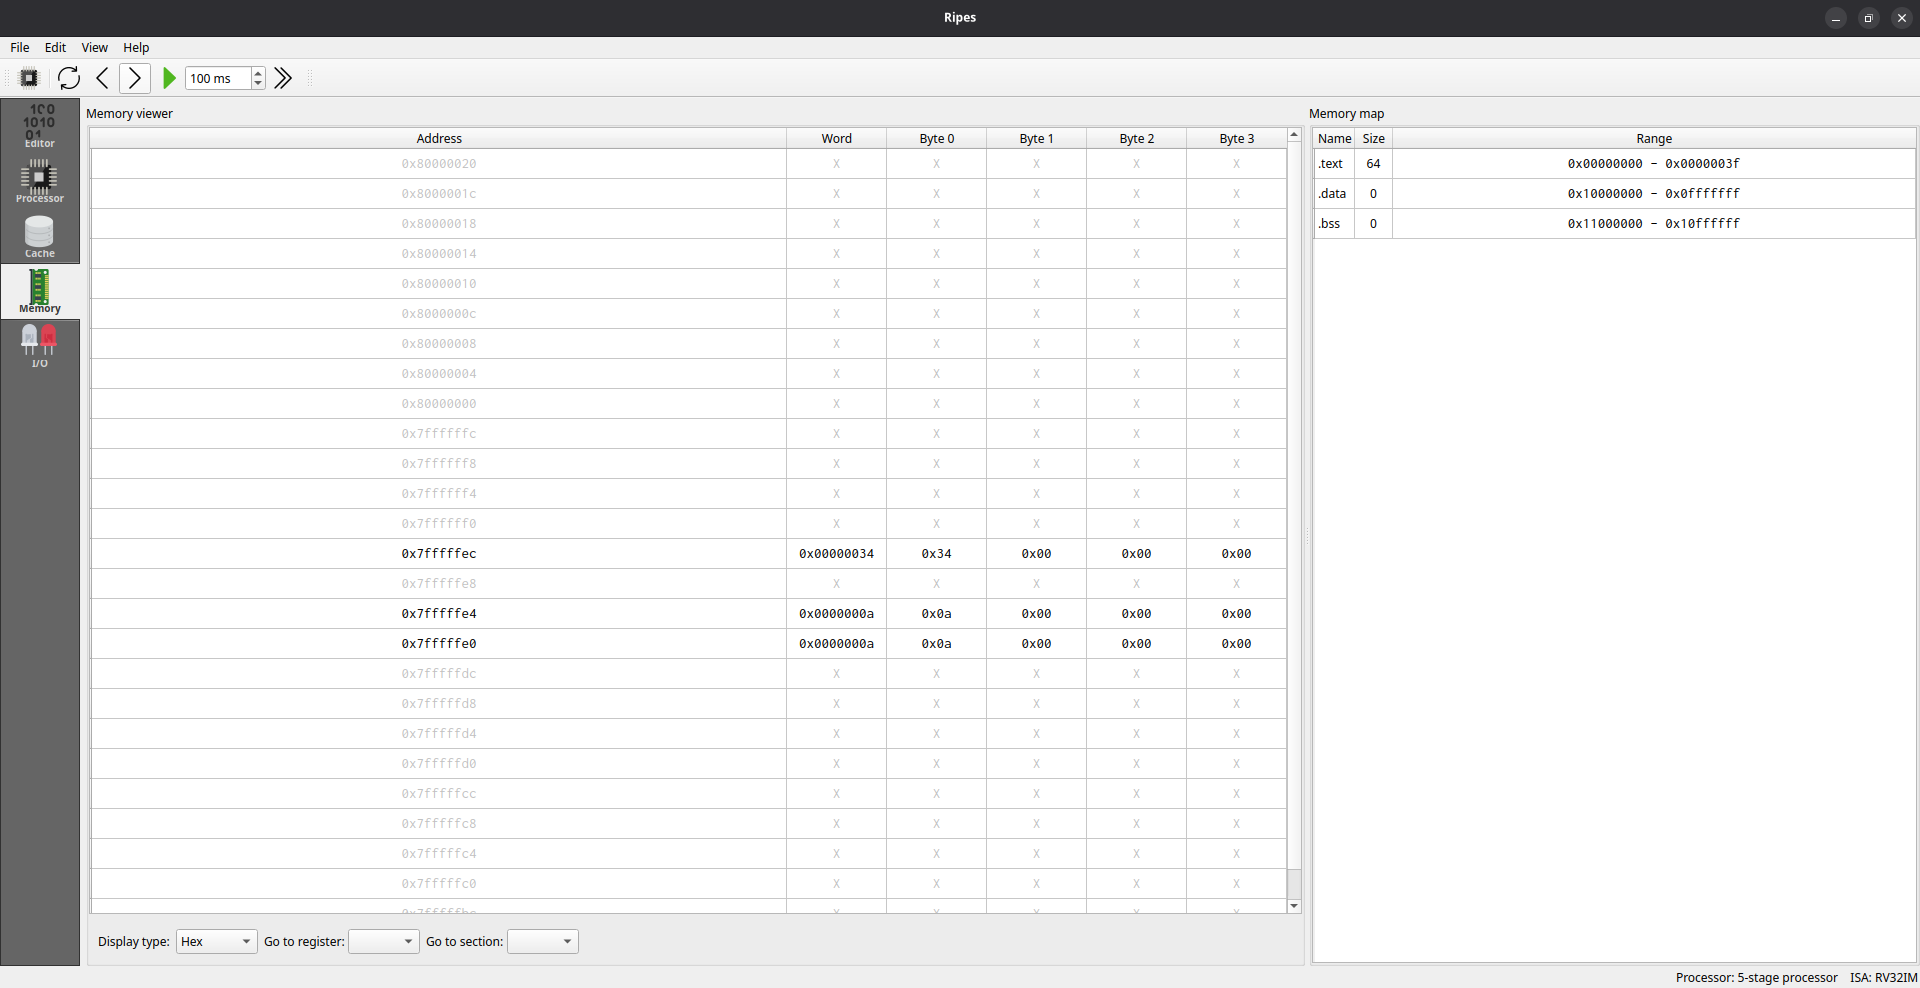
\includegraphics[width=\textwidth]{images/memory_after.png}
    \caption*{After: \texttt{sp+12 = 0x00000034}}
  \end{minipage}
  \caption{Side-by-side memory comparison showing return address corruption at sp+12.}
  \label{fig:memory_comparison}
\end{figure}

\section{Output Analysis Table}
The empirical mapping of execution states over the entirety of the attack chain is compiled below:

\begin{table}[h]
\caption{Output Analysis: Register and Memory State at Each Execution Stage}
\centering
\begin{tabular}{|c|l|l|l|}
\hline
\textbf{Stage} & \textbf{Condition} & \textbf{Register/Memory State} & \textbf{Behavior} \\
\hline
1 & Before Function Call & \texttt{ra} = return to \texttt{main} & Normal execution begins \\
2 & After \texttt{jal} & \texttt{ra} updated & Control to \texttt{vulnerable} \\
3 & Stack Setup & \texttt{sp} decreased, \texttt{ra} at \texttt{12(sp)} & Stack frame created \\
4 & Normal Buffer Write & \texttt{0(sp)}, \texttt{4(sp)} updated & Valid memory ops \\
5 & Before Overflow & \texttt{ra} in memory = original & System stable \\
6 & \textbf{After Overflow} & \textbf{\texttt{12(sp) = secret addr}} & \textbf{Return addr CORRUPTED} \\
7 & Load Return Address & \texttt{ra} = address of \texttt{secret} & Corrupted value loaded \\
8 & Function Return (\texttt{jr ra}) & \texttt{PC} = \texttt{secret} & Control flow changed \\
9 & Execution at \texttt{secret} & \texttt{t1 = 999} & Unexpected instruction \\
10 & Program End & Jump to \texttt{end} & Abnormal termination \\
\hline
\end{tabular}
\end{table}

\chapter{Discussion}

\section{Memory Integrity Violation}
In standard architectural models like RISC-V, \texttt{sp+12} serves as a protected slot exclusively designed to hold the saved return address. However, from a hardware standpoint, this data is stored in unprivileged memory. As demonstrated, there is no hardware-level segregation preventing an instruction from overwriting structural metadata. The absolute absence of runtime bounds checking represents the root vulnerability in memory corruption exploits.

\section{Control Flow Hijacking}
Control flow hijacking is defined by the unauthorized redirection of a program's execution without an explicit logic call. The test proved that by precisely targeting the stack frame and replacing \texttt{ra} from \texttt{0x00000004} to \texttt{0x00000034}, the intended architectural return mechanism becomes an arbitrary execution jump. This reflects real-world techniques such as Return-Oriented Programming (ROP) attacks.

\section{Pipeline Impact}
The manipulation of an indirect jump (\texttt{jr ra}) introduces deliberate architectural strain. Because the branch address relies on an architectural register loaded from memory, it cannot resolve during IF or ID phases. Resolution at the EX stage strictly generates a 2-cycle control hazard penalty. Specifically, the processor speculatively fetched instructions from the illicit \texttt{secret} path, revealing that the pipeline inherently trusts corrupted registers until verification occurs. 

\section{Security Implications}
Stack smashing and buffer overflows have dominated CVEs since the Morris Worm in 1988. While modern systems deploy complex layers of abstraction, this experiment proves that vulnerability fundamentally operates at the processor's most basic instruction level. RISC-V's simplified ISA clarifies this vulnerability chain: a single unrestricted store word (\texttt{sw}) instruction is sufficient to entirely subvert processor control flow.

\section{Mitigations}
Counteracting buffer overflows necessitates defense mechanisms acting on differing levels. 

\begin{table}[h]
\caption{Mitigation Strategies and Effectiveness}
\centering
\begin{tabular}{|p{3cm}|p{7cm}|l|}
\hline
\textbf{Mitigation} & \textbf{Mechanism} & \textbf{Would it Stop This?} \\
\hline
Stack Canary & Inserts a sentinel value between the buffer and \texttt{saved ra}; validated before return. & Yes \\
ASLR & Randomizes memory layout so attacker cannot know address of \texttt{secret}. & Yes \\
DEP / NX & Marks the stack as non-executable. & Partial \\
Bounds Checking & Hardware or compiler explicitly restricts \texttt{sw} operations to allocated boundaries. & Yes \\
Safe Languages & Compiler natively prevents direct memory manipulation. & Yes \\
\hline
\end{tabular}
\label{tab:mitigations}
\end{table}

\section{Limitations of the Study}
This simulation establishes the mechanical baseline of a buffer overflow under intentionally restricted conditions. The overflow evaluated was manually crafted by direct assembly instructions rather than introduced via a malicious data payload triggering a logic flaw. Furthermore, the simulation environment intentionally omits operating system privilege rings, no execution (NX) bit implementations, hardware features like superscalar execution or deep out-of-order scheduling, and complex memory hierarchies such as separate instruction and data caches. The static address mapping in Ripes also simulates an environment entirely devoid of Address Space Layout Randomization (ASLR).

\chapter{Conclusion}

This project successfully demonstrated the fundamental mechanics of a buffer overflow vulnerability using the RISC-V architecture. By constructing a targeted assembly program within the Ripes simulator, we observed the complete exploit chain: from the initial unauthorized \texttt{sw} instruction, through memory corruption, \texttt{ra} overwrite, and ultimately, \texttt{PC} hijack. 

Visual verification at each pipeline stage conclusively confirmed that corrupting the return architectural slot effectively overrides processor control flow. When the illicit \texttt{jr ra} instruction executed, the pipeline encountered an indirect branch resolution delay, causing a measurable 2-cycle control hazard penalty as it speculatively processed unintended paths. This study bridges the theoretical understanding of control hazards with practical cybersecurity exploits, underlining the critical reality that processor architectures inherently execute instructions based on register and memory states without contextual validation. Consequently, advanced mitigation mechanisms involving both software compilation checks and hardware execution restrictions remain strictly necessary to ensure systematic memory integrity.

\appendix
\chapter{RISC-V Assembly Source Code}

Below is the full, annotated RISC-V assembly source code used for the buffer overflow demonstration in the Ripes simulator. As executed, the function bypasses natural termination constraints through a stack memory violation.

\begin{lstlisting}[language=RISCV, caption={Complete Buffer Overflow Exploit Program}]
.text
.globl main

main:
    jal ra, vulnerable      # call function; ra = addr of "j end"
    j end                   # Intended return point

vulnerable:
    addi sp, sp, -16        # allocate 16-byte stack frame
    sw ra, 12(sp)           # save legitimate return address

    # --- Normal execution boundaries ---
    li t0, 10
    sw t0, 0(sp)            # buf[0] = 10
    sw t0, 4(sp)            # buf[1] = 10

    # --- Exploit Trigger ---
    # Overflow: overwrite saved return address
    la t0, secret
    sw t0, 12(sp)           # OVERFLOW: saved ra -> address of secret

    # --- Function Epilogue ---
    # Return using corrupted ra
    lw ra, 12(sp)           # ra = address of secret (corrupted)
    addi sp, sp, 16
    jr ra                   # PC hijacked -> jumps to secret

secret:
    # --- Unauthorized Execution Zone ---
    li t1, 999              # marker: proves execution reached here
    j end

end:
    nop
\end{lstlisting}


\bibliographystyle{ieeetr}
\bibliography{references}

\end{document}
